\documentclass[12pt]{article}
\usepackage{helvet}
\usepackage{graphicx}
\usepackage{geometry}
\geometry{
    a4paper,
    top = 2cm,
    left = 2cm,
    right = 2cm,
    bottom = 3cm
}
\usepackage[utf8]{inputenc}
\usepackage[spanish,mexico]{babel} % Renombra en automático los elementos a español
\addto\captionsspanish{
  \renewcommand{\figurename}{Imagen}
  \renewcommand{\tablename}{Tabla}
}
\usepackage{float}  % Etiqueta 'H' (mayus) en figuras (imágenes)
\usepackage{array}  % Padding en tablas
\usepackage{tabularx}
\usepackage{url}    % Etiqueta url en .bib
\usepackage{booktabs}   % Manejo de caudros (tablas)
\usepackage[T1]{fontenc}    % Codificación de fuentes
\usepackage[autostyle, spanish=mexican]{csquotes}       % Paquete para comillas tipográficas
\usepackage{comment}    % Comentar bloques de líneas mediante begin-end
\usepackage{multicol}   % Para poner contenido a doble columna
\usepackage{enumitem}   % Para utilizar [noitemsep, topsep=0pt] en itemize
\usepackage{amsmath}
\usepackage{mathabx} % Para testar en math mode
\usepackage{comment}
\usepackage{longtable}
\usepackage[hidelinks]{hyperref}
\usepackage{caption}
\usepackage[
  backend=biber,
  style=apa,
  sorting=nyt
]{biblatex}
\DeclareLanguageMapping{spanish}{spanish-apa}
\renewcommand{\familydefault}{\sfdefault}
\newenvironment{localsubgroup}
  {$\left\{\tabular{l}}
  {\endtabular\right.$}


\addbibresource{bibliography/00_educafi.bib}

\begin{comment}
    La tarea/manual deberá contener:

    - Portada
    - Índice o contenido
    - Desarrollo del trabajo
    - Fuente Arial 12
    - Imágenes
    - Estructura, contenido de la información, redacción y ortografía.
    - Bibliografía / Referencias electrónicas (Formato APA)
    - Conclusiones (Personales)

    Se calificará contenido y presentación del trabajo, con un mínimo de 18 hojas y un máximo de 30
\end{comment}

\begin{document}
\pagenumbering{roman}

\begin{titlepage}
  \thispagestyle{empty}
  \newgeometry{left = 1cm, right = 1cm, top = 1cm, bottom = 2cm}

  \noindent
  \begin{minipage}[c]{3.5cm}
    
\includegraphics[width=3.5cm]{media/titlepage/Escudo-UNAM.pdf}
  \end{minipage}\hfill
  \begin{minipage}[c][3.5cm][c]{\dimexpr\textwidth-7cm\relax}
    \centering
    {\large\textbf{Universidad Nacional Autónoma de México}\\[0.6em] 
    \Large\textbf{Facultad de Ingeniería}\\[0.6em]
    \large Sistemas Operativos}
  \end{minipage}\hfill
  \begin{minipage}[c]{3.5cm}
    \raggedleft
    
\includegraphics[width=3.5cm]{media/titlepage/FI.png}
  \end{minipage}
\centering\huge
  \vfill
    Grupo 1 \\
    Ing. Angel Isidro Mercado
  \vfill
    \textbf{Tarea Registro en sistema EDUCAFI}
  \vfill\large
    320304435 - Cabrera Rojas Oscar
  \vfill

  \noindent\footnotesize \hfill Ciudad Universitaria, CDMX a 26 de agosto del 2026
\end{titlepage}
\restoregeometry

\tableofcontents

\pagenumbering{arabic}
\setcounter{page}{1}

\section{Evidencia}

\begin{figure}[H]
    \centering
    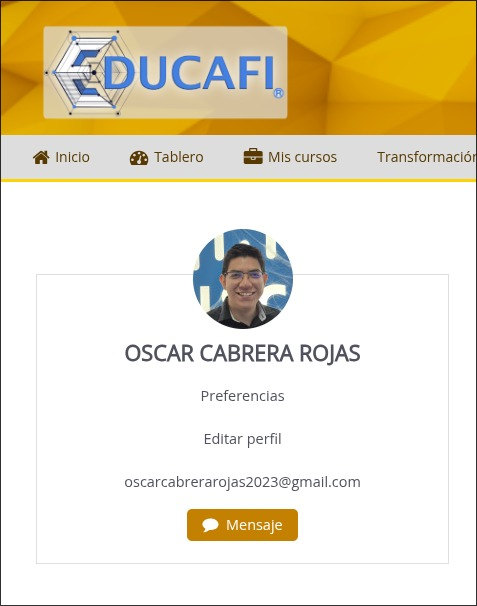
\includegraphics[width=0.7\textwidth]{media/t00/foto_perfil.jpeg}
    \caption{Evidencia de la actualización sobre la foto de perfil en la plataforma de EDUCAFI.\cite{educafi03}}
    \label{fig:foto-perfil}
\end{figure}

\section{Conclusiones}

La actualización de datos personales implica la aceptación de los lineamientos y forma de trabajo del curso, así como la declaración de concordancia de identidad por parte del alumno. Que sea una actividad previa a las tareas numeradas es la decisión de planeación correcta para iniciar las actividades del semestre.

\nocite{*}
\printbibliography[heading=bibintoc, title={Referencias}]

\end{document}